\section{Pruning Search Space of Symbolic Execution}
Recent and impressive progress in constraint solvers as well as the combination of both concrete and symbolic execution (referred as concolic execution~\cite{cute,compositional} or mixed execution~\cite{mixed}) make it possible to perform automatic path-based testing on large scale programs. However, these technologies are still suffering from two major bottlenecks: efficient constraint solving and the path explosion phenomenon. S\'{e}bastien Bardin and Philippe Herrmann~\cite{prune} focus on the second issue and propose three complementary heuristics geared toward lowering path explosion. All these heuristics deal with different distinct sources of path explosion. 

To cover all paths of a program is not the primarily objective of current testing practices. Often the case, it is only required to fully cover a class of structural artifacts of the program code source, such as statements, branches or atomic predicates. In the rest of the section, we denote these three classes of artifacts as structural coverage. There is an obvious mismatch between path-based approaches and such item coverage goals: while each new test data does cover a new path, it may hit no new item. Thus, path-based testing methods tend to waste a lot of time trying to compute irrelevant test data, i.e. test data exercising no new structural coverage. 


To address the path explosion issue in path-based testing with item coverage objectives, they provide three heuristics to discard irrelevant paths as much as possible, reducing of the number of solver calls and the whole computation time. The three heuristics are used as enhancements of a (bounded) depth-first search (DFS) path-based procedure, either purely symbolic or concolic. Original path-based testing techniques were based on DFS~\cite{dart,cute, onthefly}, while some recent works advocate using other search strategies~\cite{exe,hybrid,fuzz}.

\subsection{Look-Ahead heuristic}
\begin{figure}
\centering
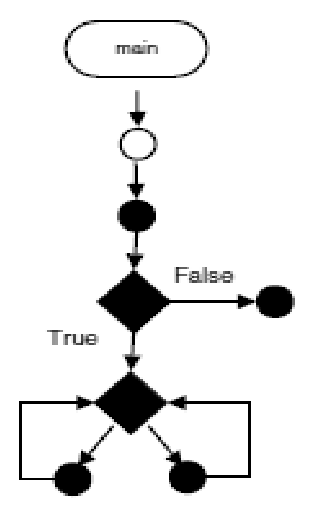
\includegraphics[scale=0.35,clip]{fig/la.eps} 
\caption{\label{fig:la}Example of Look-Ahead (LA) Heuristic} 
\end{figure}

The key idea of the Look-Ahead (LA) heuristic is to perform a reachability analysis in terms of reachable items in the CFG, and decide whether the current
path must be expanded based on the reachability analysis. If no new items can be reached, then exploration along the current path is stopped.

Figure \ref{fig:la} shows an example for illustrating the Look-Ahead (LA) heuristic. Let us assume the depth bound $k \geq 4$ and the objective is to achieve full statement coverage, and every path of the program is feasible. Then the original DFS based produre needs to explore $\approx2^k$ paths to achieve full coverage (because of the two nested loops) while DFS+LA requires at most 3 paths: one path to cover the false branch and two paths to cover two loops.

\subsection{Max-CallDepth (MCD) heuristic}
The major source of path explosion is function calls, and especially nested function calls. It is more embarrassing when only the top-level function is of interest. For example, it may be the case that the procedure explores alternative (long) paths due to backtrack in deep callees while a simple backtrack at top-level would be sufficient. Example of figure \ref{fig:mcd} gives such a behaviour.

\begin{figure}
\centering
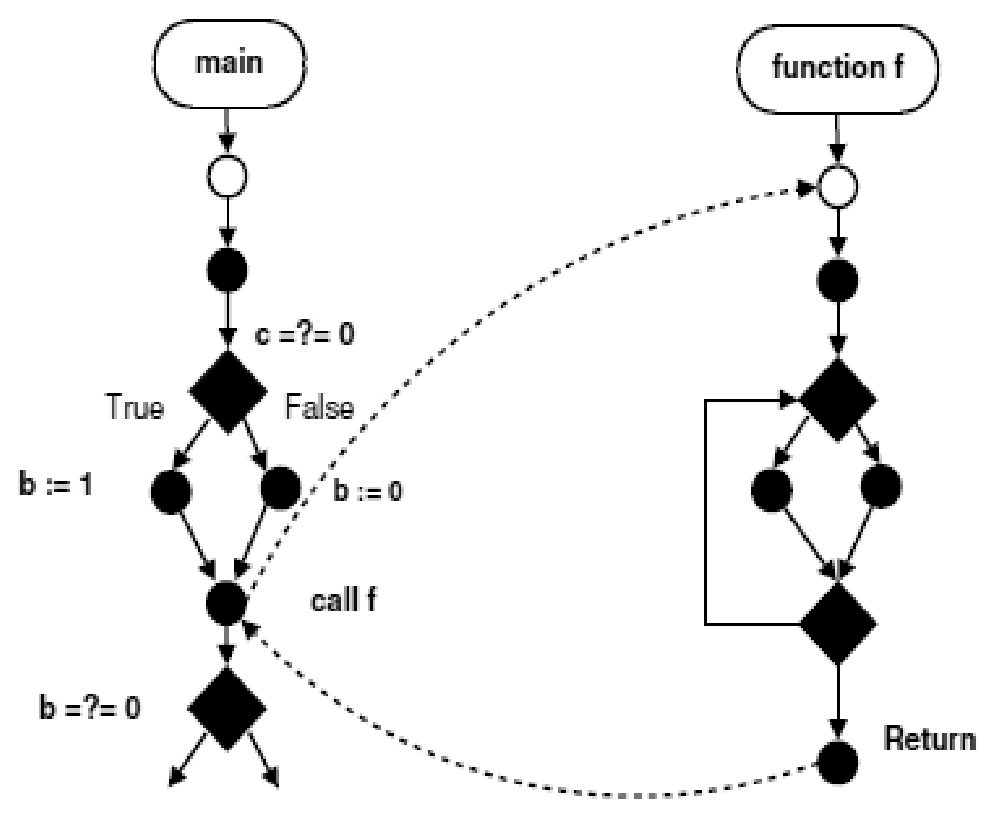
\includegraphics[scale=0.35,clip]{fig/mcd.eps} 
\caption{\label{fig:mcd}Example of Max-CallDepth (MCD) heuristic} 
\end{figure}

The principle of the Max-CallDepth heuristic (MCD) is to prevent backtracking in deep nested calls, hoping such a deep decision is not mandatory to cover the function under test. It is clear that this heuristic makes sense only in unit testing. Moreover, contrary to LA, MCD may discard relevant paths and prevent the full coverage of the function under test. On the other hand, on some programs MCD can discard many paths and still achieve full coverage. These results are summarised in the next property.

\subsection{Solve-First (SF) heuristic}


